%
%  hume.four
%
%  Created by Mark Eli Kalderon on 2007-08-04.
%  Copyright (c) 2007 Mark Eli Kalderon. All rights reserved.
%
%  Beamer

% Definitions and macros
\newcommand{\change}{\textcolor{blue}{\textbf{CHANGE SLIDE}}}
\newcommand\myauthor{Mark Eli Kalderon} 
\newcommand\mytitle{Introduction to Moral Philosophy}
\newcommand\mysubtitle{Hume}
\newcommand\myinstitution{University College London}
\newcommand\myurl{http://markelikalderon.com/teaching/}

% Packages specific to lecture notes
\mode<article>{
    \usepackage{palatino}
}

% Packages specific to beamer presentation
\mode<presentation>{
    \usetheme{Darmstadt}
    \setbeamercovered{transparent}
    \pgfdeclareimage[height=0.5cm]{university-logo}{../../graphics/logo_sml_blk}
    \logo{\pgfuseimage{university-logo}}
}

% Packages common to lecture notes and beamer presentation
\usepackage{pgf}
\usepackage{tikz}
\usepackage{hyperref}

\setjobnamebeamerversion{hume.four.beamer}

\title{\mytitle}
\subtitle{\mysubtitle}

\author{\myauthor\\
\url{\myurl}}
\institute{\myinstitution}

% \date[Short Occasion] % (optional)
% {Date / Occasion}

\begin{document}

\frame{\maketitle}

\section{Main Points from Last Time}\label{sec:main_points_from_last_time} % (fold)

% TODO: Add opening remarks

\change\ Last time we finished discussing Hume's philosophical psychology and began discussing its implications for the distinction between vice and virtue. One claim of Hume's philosophical psychology presently relevant to his account of the distinction between vice and virtue is the claim that reason alone can neither determine the will nor oppose the passions' determination of the will. Two considerations were prominent in establishing this claim. The first consideration involved a positive characterization of reason's proper office. The faculty of reason is confined to two operations:
\begin{itemize}
	\item Reason may \emph{demonstrate} certain truths based on the relations among our ideas (such as the truths of logic and mathematics).
	\item Reason may \emph{infer}, or render probable, on the basis of experience, that the relations of cause and effect obtain between objects and events.
\end{itemize}
The problem is that neither operation unsupplemented by an attendant purpose which only a passion could provide could determine the will. One weakness of this argument is that it would fail to persuade those who denied that reason was so confined to these operations. The second consideration forms the basis of an argument not susceptible to this weakness. Recall that passions are simple impressions of reflection that arise under certain conditions and that prompt us to occassion further ideas and impressions and to act in certain ways. The passions are ``original existences'', and so cannot represent anything. According to Hume, for a thing to have a representative quality it must be the ``copy of another existence'', but the passions, being original existences are the copy of no other thing. (This argument invokes Hume's first principle of the science of human nature---that simple ideas are copies of impressions they resemble.) Since the passions do not represent anything, they cannot contradict a truth discovered by reason. And if the passions cannot contradict a truth discovered by reason, reason can never oppose the passions' determination of the will.

Hume also provides a diagnosis for why the image of reason's combat with the passions has long held sway among philosophers and the vulgar alike. Specifically, we are apt to confuse the operation of the calm passions for the operation of reason. The calm passions, like reason, acts with little sensible emotion and occasion no disorder. In this way, the calm passions contrast with the violent emotions that act with strong emotion and tend to occassion disorder. What the vulgar denominate as the combat of reason and the passions is really the conflict of certain calm and violent emotions.

These results in philosophical psychology are germane to a longstanding dispute in moral philosophy between moral rationalists and moral sentimentalists. Moral rationalists held that moral judgments are determined by reason, whereas moral sentimentalists held that moral judgments are determined by internal sentiment. Within Hume's framework this debate turns on the question whether it is by means of our ideas or impressions that we can distinguish between vice and virtue and pronounce an action blameable or praise-worthy. With the debate between the rationalists and sentimentalists understood in this way, Hume offers two main arguments against moral rationalism. First moral distinctions influence the will and so could not be determined by reason since the will is and ought only to be the slave of the passions. The second argument consists in a piece of abstruse reasoning. If reason determines the distinction between vice and virtue it must do so on the basis of the relations of ideas. However, there are no relations which reason can determine the vice or virtue of an action, sentiment, or character. \change

% \textbf{See Figure~\ref{fig:slide0}.}
% 
% \begin{figure}[ht]
%     \begin{center}
%         \includeslide[height=5cm]{slide0<1>}
%     \end{center}
%     \caption{Caption}
%     \label{fig:slide0}
% \end{figure}

\frame<presentation>[label=slide0]{
    \frametitle{Main Points from Last Time}
        \begin{columns}
            \begin{column}{3cm}
                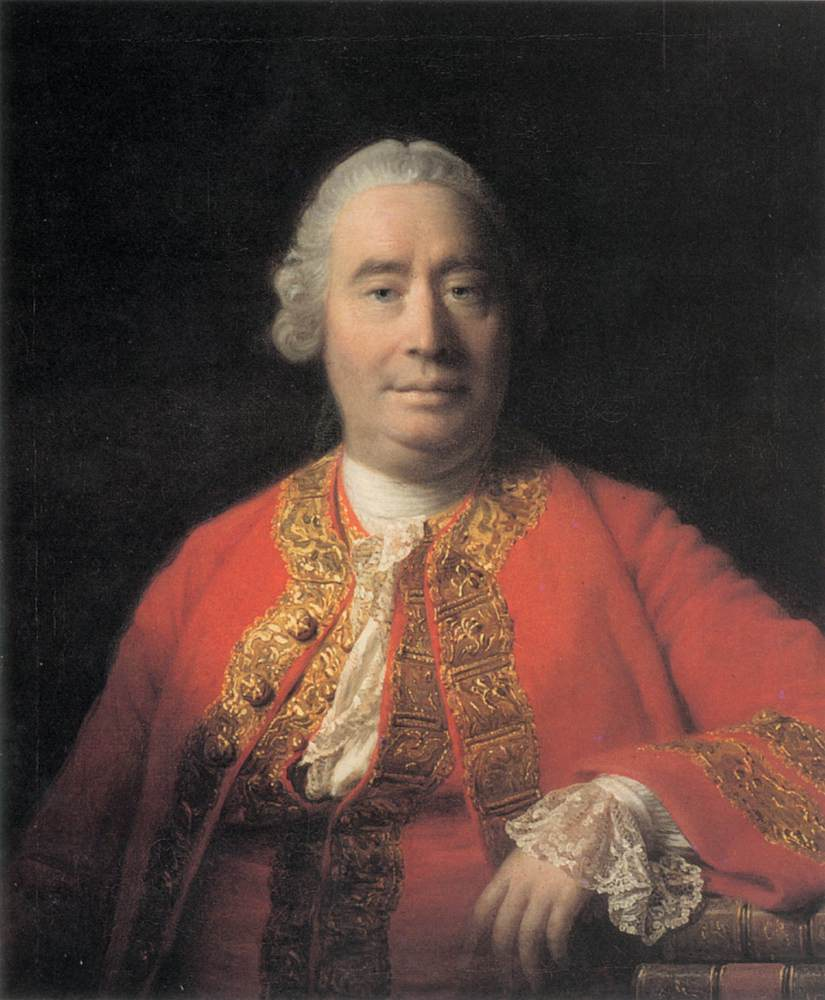
\includegraphics[height=4cm]{../../graphics/hume.jpg}
            \end{column}
            \begin{column}{7cm}
                \begin{itemize}
                    \item Reason alone can neither determine the will nor oppose the passions' determination of the will
                    \item The vulgar in thinking otherwise conlfate the operation of the \alert{calm passions} with the operation of \alert{reason}
                    \item Moral distinctions influence the will and so cannot be determined by reason
                    \item There are no relations from which reason can determine the virtue or vice of an action, sentiment, or character
                \end{itemize}
            \end{column}
        \end{columns}
}

Let's briefly review this argument since the details will be presently relevant. If moral distinctions are really demonstrable by reason, then we must be able to discern them on the basis of one or more of four specific relations---resemblance, contrariety, comparison in degress in quality, and proportions in quantity and number. Moral distinctions pertain exclusively to our actions, passions, and characters. However, the four demonstrable relations obtain not only among our actions, passions, and characters, but among inanimate obects as well. So the distinction between vice and virtue cannot be demonstrated on the basis of them. What if the moral rationalist maintains, contra Hume, that moral distinctions are demonstrable on the basis of some \emph{further} relation. (Thus Clarke speaks of the relations of \emph{fitingness} and \emph{unfitingness} that virtuous and vicious actions bear to the circumstances in which they are performed.) If the moral rationalist is tempted to make this reply, Hume contends that he must explicitly specify the novel relations and do so subject to two conditions:
\begin{itemize}
    \item First, the relations must obtain between perceptions in the mind and external objects.
    \item Second, the relations, being demonstrable, are knowable a priori and cause everyone that knows them to act virtuously to some degree.
\end{itemize}
Hume doubt, however, whether either condition could be met. First he doubts whether a relation that obtained between a perception and an external object could not also obtain among perceptions alone, or among external objects alone. Second, he observes that it is not enough that a subject comes to know of a moral distinction on the basis of the obtaining of some relation, but in so knowing he must have a tendency to act accordingly. However, he doubts whether there could be any proof of this further necessary connection between the knowledge of the relations and the will.

% \textbf{See Figure~\ref{fig:slide1}.}
% 
% \begin{figure}[ht]
%     \begin{center}
%         \includeslide[height=5cm]{slide1<1>}
%     \end{center}
%     \caption{Hume's Second Argument}
%     \label{fig:slide1}
% \end{figure}

\frame<presentation>[label=slide1]{
    \frametitle{Hume's Second Argument}
            \alert{P1} If moral distinctions are not demonstrable, they must be so on the basis of the relations of ideas\\
            \alert{P2} Moral distinctions are not demonstrable on the basis of the four relations\\
            \alert{P3} If they are demonstrable on the basis of a novel relation, the relation must meet two conditions: (i) it must obtain between perceptions and objects; (ii) it must causally affect everyone in the same way\\
            \alert{P4} No relation could meet these two conditions\\
            \alert{C} Therefore, moral distinctions are not demonstrable
}


% section main_points_from_last_time (end)

\section{Hume's examples}\label{sec:hume_s_examples} % (fold)

This second argument is a piece of abstruse reasoning that may silence without convincing the moral rationalist. Hume recognizes this difficulty and addresses it by presenting the reader with concrete examples of vice. In reflecting on the moral judgments that these examples elicit, the reader can confirm for himself that moral distinctions are determined not by reason but by internal sentiment.

Hume discusses two kinds of example corresponding to the two operations of reason:

\begin{itemize}
	\item Reason may \emph{demonstrate} certain truths based on the relations among our ideas (such as the truths of logic and mathematics).
	\item Reason may \emph{infer}, or render probable, on the basis of experience, that the relations of cause and effect obtain between objects and events.
\end{itemize}

In demonstrating a truth, reason compares ideas and determines the relations that obtain among them. If something is vicious and this is demonstrable by means of certain relations among ideas, then whenever these same relations obtain, something must be vicious. If something failed to be vicious though these same relations obtain, then vice could not consist in these relations among ideas. Hume tries to convince the reader of this by considering an uncontroversial example of vice:

\begin{quote}
	Of all crimes that human creatures are capable of committing, the most horrid and unnatural is ingratitude, especially when it is committed against parents, and appears in the more flagrant instances of wounds and death. (\emph{Treatise}, 3.1.1.24)
\end{quote}

But the relations that obtain in cases of parricide may also obtain among inanimate objects in cases that manifestly involve no vice. Hume asks us to consider the example of a tree that produces a sapling that overtops it and destroys the parent tree. Observe that the tree and the sapling bear the same relations as parent and child in the case of parricide. However, whereas parricide is manifestly vicious, the sapling's destroying the parent tree is manifestly not. So reason could not demonstrate parricide to be vicious on the basis of these relations. Hume's second example of this kind is the uncontroversial vice of human incest. Observe that the relations that obtain in cases of human incest also obtain in cases of nonhuman incest. However, whereas human incest is manifestly vicious, nonhuman incest is manifestly not. So reason could not demonstrate human incest to be vicious on the basis of these relations.

Not only does reason demonstrate truths by comparing ideas and determining the relations that obtain among them, but reason may also infer matters of fact on the basis of experience. Hume asks us to consider the case of willful murder, and observe the matters of fact in that case:

\begin{quote}
	Examine it in all lights, and see if you can find that matter of fact, or real existence, which may be called vice. In which-ever way you take it, you find only certain passions, motives, volitions, and thoughts. There is no other matter of fact in the case. The vice entirely escapes you, as long as you consider the object. (\emph{Treatise}, 3.1.1.26)
\end{quote}

If the vice of willful murder does not consist in any matter of fact and real existence discoverable by reason, then how is the manifest vice of willful murder determined by the human mind? If we cautiously observe what transpires as we engage in the imaginative exercise that Hume prescribes, we will discover that the vice is determined by an internal sentiment of disapprobation that is annexed to our idea of willful murder:

\begin{quote}
	You never can find it, till you turn your reflection into your own breast, and find a sentiment of disapprobation, which arises in you, towards this action. Here is a matter of fact; but 'tis the object of feeling, not of reason. It lies in yourself, not in the object. So that when you pronounce any action or character to be vicious, you mean nothing, but that from the constitution of your nature you have a feeling or sentiment of blame from the contemplation of it. (\emph{Treatise}, 3.1.1.26)
\end{quote}

Reason has two kinds of operations: (i) demonstrating truths on the basis of relations among ideas and (ii) inferring matters of fact on the basis of experience. Vice (and by implication virtue) could not be determined by relations among ideas nor by inferred matter of fact. Since these exhaust the operations of reason it follows that reason could not determine our judgments of virtue and vice.

Hume's second kind of case---the case of willful murder---provides an independent reason for this conclusion. In imagining an instance of willful murder we can observe that our sense of its vice arises in the disapprobation we feel towards it. Not only does reflection on the case of willful murder help to establish Hume's negative claim---that moral distinctions are not determined by reason, such reflection also establishes Hume's positive claim---that moral distinctions are determined by internal sentiment. Not only does such reflection establish the falsity of moral rationalism, but such reflection also establishes the truth of moral sentimentalism. \change

% \textbf{See Figure~\ref{fig:slide2}.}
% 
% \begin{figure}[ht]
%     \begin{center}
%         \includeslide[height=5cm]{slide2<1>}
%     \end{center}
%     \caption{Hume's Examples}
%     \label{fig:slide2}
% \end{figure}

\frame<presentation>[label=slide2]{
    \frametitle{Hume's Examples}
        Hume's examples correspond to the two operations of reason:
        \begin{itemize}
        	\item Reason may \emph{demonstrate} certain truths based on the relations among our ideas (such as the truths of logic and mathematics).
        	\item Reason may \emph{infer}, or render probable, on the basis of experience, that the relations of cause and effect obtain between objects and events.
        \end{itemize}
}

% section hume_s_examples (end)

\section{The Moral Sense}\label{sec:the_moral_sense} % (fold)

Moral judgments are perceptions in the human mind. Perceptions are impressions or ideas but not both. So if moral judgments are not ideas, as Hume has argued, then they must be impressions. So Hume concludes that ``[m]orality, therefore, is more properly felt than judg'd of'' (\emph{Treatise}, 3.1.2.1). Though rationalists are mistaken, their mistake is explicable. The sentiments by which morality is felt are often calm. Since calm sentiments have little sensible emotion they are apt to be confounded with ideas which they resemble in this respect.

If moral distinctions, particular judgments of virtue and vice, are impressions, what kind of impressions are they? According to Hume, virtue produces in the human mind an agreeable impression of pleasure, whereas vice produces in the human mind a disagreeable impression of pain:

\begin{quote}
	virtue is distinguish'd by the pleasure, and vice by the pain, that any action sentiment or character gives us by the mere view and contemplation. (\emph{Treatise}, 3.1.2.11)
\end{quote}

First, notice that, for Hume, the objects of moral evaluation, the kinds of things that can be properly judged virtuous or vicious are actions, sentiments, and characters (understood as more or less stable configuration of passions). Later Hume will importantly qualify this: Actions may be judged virtuous or vicious but only \emph{derivatively}---an action is virtuous or vicious only if its motive is virtuous or vicious. Second, notice that the pleasure and pain by which something is judged virtuous or vicious arises upon its contemplation. Later Hume will importantly qualify this as well: It is only pleasure or pain \emph{upon the general view or survey} that distinguishes virtue and vice. \change

% \textbf{See Figure~\ref{fig:slide3}.}
% 
% \begin{figure}[ht]
%     \begin{center}
%         \includeslide[height=5cm]{slide3<1>}
%     \end{center}
%     \caption{The Moral Sense}
%     \label{fig:slide3}
% \end{figure}

\frame<presentation>[label=slide3]{
    \frametitle{The Moral Sense}
        \begin{columns}
            \begin{column}{3cm}
                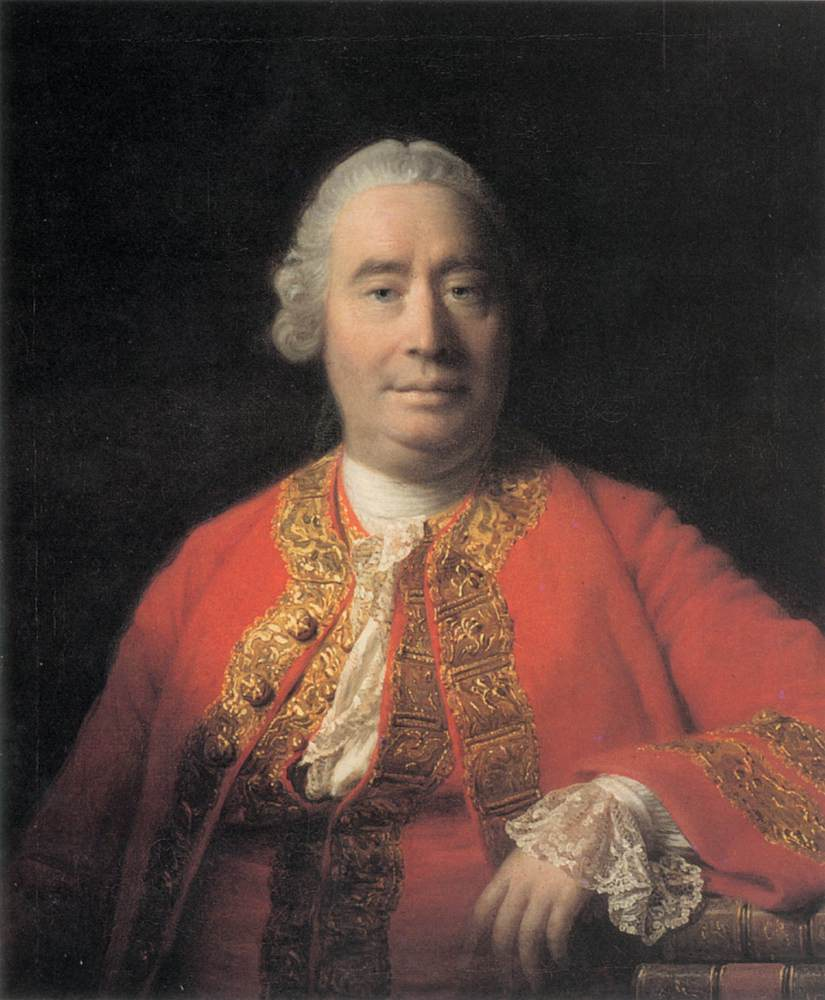
\includegraphics[height=5cm]{../../graphics/hume.jpg}
            \end{column}
            \begin{column}{7cm}
                Virtue is distinguish'd by the pleasure, and vice by the pain, that any action sentiment or character gives us by the mere view and contemplation. (\emph{Treatise}, 3.1.2.11)
            \end{column}
        \end{columns}
}

There is a potential difficulty with this sentimentalist proposal that parallel's a difficulty that Hume raised for moral rationalism. In maintaining that virtue and vice consists in certain relations discernible by reason, rationalists are committed to the existence of virtue or vice wherever these relations obtain. The problem is that these relations obtain among inanimate objects, but only objects that can act and have sentiments and stable characters could be the objects of moral evaluation. But notice that we take pleasure and pain in inanimate objects, and so it can seem that sentimentalism faces the same difficulty that moral rationalism faced: Wrongly classifying inanimate objects as objects of moral evaluation.

However, Hume believes that sentimentalism has two replies unavailable to the rationalist:

\begin{itemize}
	\item The particular pleasure or pain that we feel in judging of virtue and vice differs in kind from the pleasures or pains that we feel in response to things that are not the objects of moral evaluation.
	\item The particular pleasure or pain that we feel in judging of virtue and vice occasion the passions of pride and humility, love and hatred, but not all pains or pleasures we feel towards things that are not objects of moral evaluation can give rise to these passions.
\end{itemize}

First, the particular pleasure or pain that we feel in judging of virtue and vice differs in kind from the pleasures or pains that we feel in response to things that are not the objects of moral evaluation. The pleasure we take in music is not the same kind of pleasure that we take in a good bottle of wine. Just as we take distinctive pleasures in music and wine, Hume suggests that we take a distinctive pleasure in virtue. A virtuous action, sentiment, or character may occasion a particular pleasure, but this pleasure differs in kind from the particular pleasures occasioned by inanimate objects such as musical compositions and good bottles of wine.

Second, the particular pleasure or pain that we feel in judging of virtue and vice occasion the passions of pride and humility, love and hatred, but not all pains or pleasures we feel towards things that are not objects of moral evaluation can give rise to these passions. Recall that pride and humility and love and hatred are indirect passions that arise from the double relation of ideas and impressions. Whereas pride is an agreeable impression that takes the self as its object, love is an agreeable impression that takes another as its object. And whereas humility is a disagreeable impression that takes the self as its object, hate is a disagreeable impression that takes another as an object. If we classify indirect passions by whether they are agreeable or disagreeable and whether they take the self or the other as their object, we can taxonomize these passions as follows:

Virtue and vice involve agreeable and disagreeable impressions---they occasion a particular pleasure or pain. Moreover, the objects of moral evaluation are actions, sentiments, and characters, and these belong to either to oneself or another. Thus the moral pleasure that a person might take in his own character, through the double relations of ideas and impressions, occasions the passion of pride. Specifically, since it is the person's character that is the object of moral pleasure, by the natural association of ideas, this will tend to occasion the person's idea of himself. Since the moral pleasure resembles the pleasure of pride, by the natural association of impressions, this will tend to occasion the pleasure of pride. Later, Hume will classify virtues as whether they are useful or agreeable to self or to others. Correspondingly, Hume would classify vices as whether they are useless (or, rather, counterproductive) or disagreeable to self or to others. If we classify virtue and vice by whether they are agreeable or disagreeable and whether they take the self or the other as their object, we can taxonomize these on the model of the square of passions.

Not every inanimate object gives rise to these indirect passions. If the good bottle of wine that I take pleasure in is not proper to me and so does not occasion my idea of myself it will not give rise to pride. While not all things that fail to be the objects of moral evaluation give rise to the indirect passions, some do. So Hume's second response to the difficulty of wrongly classifying inanimate objects as virtuous or vicious is incomplete. How do we distinguish the cases where the pleasures and pains that give rise to the indirect passions are moral approbation and disapprobation from those where they are not? Perhaps the answer to this question has to do with the nature of the circumstances that occasion the pleasure or pain---it is the pleasure and pain occasioned \emph{upon the general view or survey} of an action, sentiment, or character that morality is judged of.

Since moral judgments just are particular pains or pleasures occasioned upon the general view or survey, to explain our moral judgments it suffices to explain the circumstances that occasion moral approbation and disapprobation. Recall that one advantage that Hume claims for his account of the passions is that they are governed by a few general principles rather than explaining each in terms of an original impulse. It is the way in which Hume can explain the multiplicity of observed phenomena with respect to the human passions in terms of a few general principles that makes it the paradigm of his new science of human nature. Hume also claims a similar advantage for his brand of moral sentimentalism:

\begin{quote}
	For as the number of duties is, in a manner, infinite, 'tis impossible that our original instincts shou'd extend to each of them, and from our very first infancy impress on the human mind all that multitude of precepts, which are contain'd in the compleatest system of ethics. (\emph{Treatise}, 3.1.2.6)
\end{quote}

Just as Hume explains the multiplicity of observed phenomena with respect to human passions in terms of a few general principles, Hume explains the multiplicity of observed phenomena with respect to human morality in terms of a few general principles. It is this further success of the new science of human nature that explains the upbeat character of the conclusion of Book III which contrasts so markedly with the note of despair upon which Book I concludes. \change

% \textbf{See Figure~\ref{fig:slide4}.}
% 
% \begin{figure}[ht]
%     \begin{center}
%         \includeslide[height=5cm]{slide4<1>}
%     \end{center}
%     \caption{A potential difficulty}
%     \label{fig:slide4}
% \end{figure}

\frame<presentation>[label=slide4]{
    \frametitle{A Potential Difficulty}
        Wrongly classifying inanimate objects as virtuous or vicious. Two responses:
        \begin{itemize}
        	\item The particular pleasure or pain that we feel in judging of virtue and vice differs in kind from the pleasures or pains that we feel in response to things that are not the objects of moral evaluation.
        	\item The particular pleasure or pain that we feel in judging of virtue and vice occasion the passions of pride and humility, love and hatred, but not all pains or pleasures we feel towards things that are not objects of moral evaluation can give rise to these passions.
        \end{itemize}
}

% section the_moral_sense (end)

\section{Natural and Artificial Virtues}\label{sec:natural_and_artificial_virtues} % (fold)

Since moral distinctions just are particular pains or pleasures occasioned upon the general view or survey, to explain our distinctions between virtue and vice it suffices to explain the circumstances that occasion moral approbation and disapprobation. Are the principles that explain moral pleasures and pains natural? According to Hume, this question has no straightforward answer since distinct senses of ``natural'' can be distinguished:

\begin{itemize}
    \item In one sense, natural contrasts with \emph{miraculous}. Not only is the distinction between virtue and vice natural in this sense, but so is everything else ``\emph{excepting those miracles, on which our religion is founded}'' (\emph{Treatise}, 3.1.2.7).
    \item In another sense, natural contrasts with \emph{unusual}. The distinction between virtue and vice is natural in this sense. Hume observes that there never was a nation in the world nor a single person in any nation, who was utterly lacking in the moral sense (\emph{Treatise}, 3.1.2.8).
    \item In another sense, natural contrasts with \emph{artificial}. It is important to recognize the intended contrast. Natural, here, is not being contrasted with the unreal or fake, but rather with what is the product of human artifice. Hume claims that while certain virtues such as benevolence are natural, other virtues such as justice are artificial. While the moral approbation we feel towards benevolent acts is natural, the moral approbation we feel towards just acts is partly the result of artifice and human convention.
\end{itemize}

Natural virtues include benevolence, generosity, charity, love of life, and kindness to children. Artificial virtues include justice, fidelity, honesty, and chastity.

% \begin{figure}[ht]
%     \begin{center}
%         \includeslide[height=5cm]{slide5<3>}
%     \end{center}
%     \caption{Is Morality Natural?}
%     \label{fig:slide5}
% \end{figure}

\frame<presentation>[label=slide5]{
    \frametitle{Is Morality Natural?}
        \begin{columns}
            \begin{column}{3cm}
                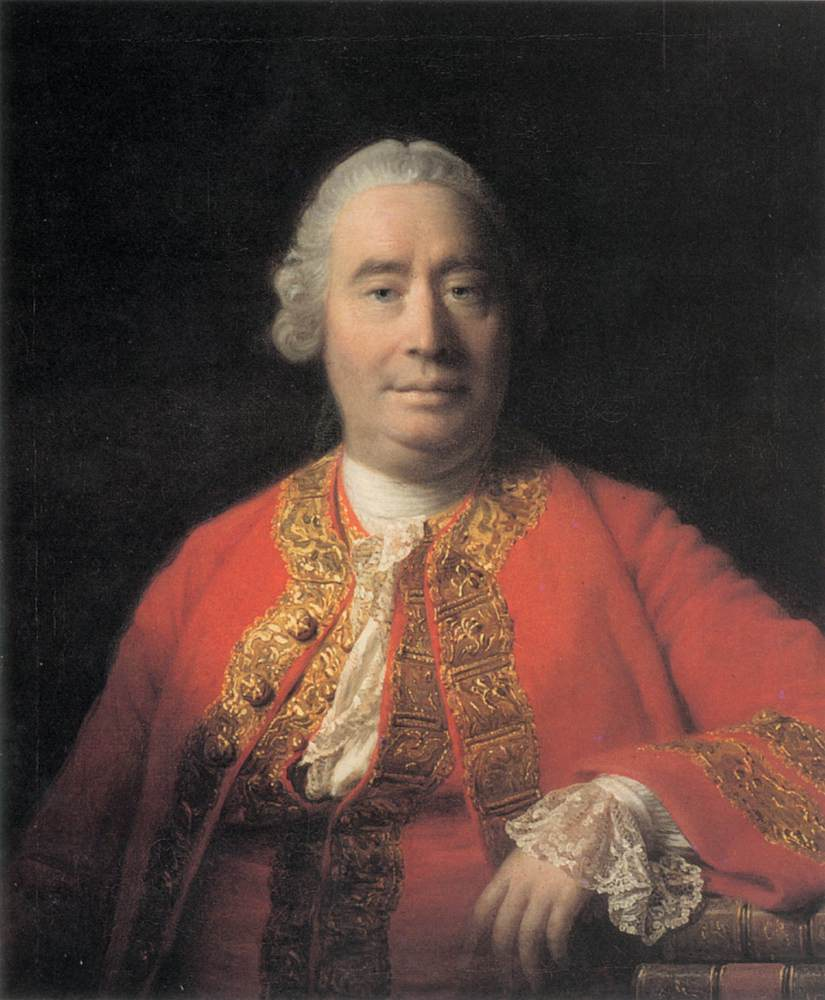
\includegraphics[height=4cm]{../../graphics/hume.jpg}
            \end{column}
            \begin{column}{7cm}
                Depends on what you mean by natural. Three contrasts"
                \begin{itemize}
                    \item<1-> Natural vs \alert{miraculous}
                    \item<2-> Natural vs \alert{unusual}
                    \item<3-> Natural vs \alert{artificial} (not fake, but the product of artifice)
                \end{itemize}
            \end{column}
        \end{columns}
}

Natural virtues have two important features:

\begin{enumerate}
	\item First, natural virtues are implanted instincts. They involve behavioral dispositions native to human beings. More specifically, they involve natural dispositions to perform certain types of actions under certain types of circumstances. So, for example, the natural virtue of kindness to children involves the disposition to feed a child if the child is hungry.
    \item Second, the manifestation of natural virtue invariably results in good. Each performance of the relevant type of action in the relevant type of circumstance results in some good. So for example, when kindness moves us to feed a hungry child, this action results in some good---the hunger of the child is abated.
\end{enumerate}

In contrast, the artificial virtues differ in both these respects from the natural virtues:

\begin{enumerate}
	\item First, the artificial virtues are not implanted instincts. Rather the artificial virtues involve dispositions to behave in accordance with a general scheme or convention, itself a product of human artifice. Observances of the general scheme are too various and complex for each to be the result of a distinct behavioral disposition native to human beings.
    \item Second, the manifestation of artificial virtue does not invariably result in good. It is not the case that every observance of the general scheme benefits either the private individual or the public. Justice, for example, may require us to repay a debt to an enemy or to someone who will use the funds to some malicious end contrary to the public good. It is the general compliance with the scheme or convention that benefits the public and not any particular observance of that general scheme.
\end{enumerate}

Justice is Hume's central example of an artificial virtue. In the first section of part two, Hume establishes his main negative conclusion: Hume argues that justice could not be a natural virtue. In the second section of part two, Hume gives his positive account of justice as an artificial virtue.
Hume's positive account has two stages. The first stage is a genealogy of justice: Hume explains the motives and circumstances that first established the conventions of justice. The second stage is an account of the moral beauty of just acts: Hume gives a separate explanation for why observances of these conventions have merit and are the proper object of moral approbation. Notice that the original motive to justice is not the principle that bestows merit upon just acts, that is, particular observances of the general scheme.
This is an important further difference between natural and artificial virtues. With respect to the natural virtues, the motive to virtuous action is what bestows merit upon that action. Consider kindness to children. When you feed a hungry child, the motive is kindness, and it is the amiableness of this action, its being motivated by kindness, that bestows merit upon the action and makes it the object of moral approbation. With artificial virtues, however, the original motive for virtuous action is distinct from the principle that bestows merit upon the action and makes it the object of moral approbation.

% \textbf{See Figure~\ref{fig:slide6}.}
% 
% \begin{figure}[ht]
%     \begin{center}
%         \includeslide[height=5cm]{slide6<4>}
%     \end{center}
%     \caption{Caption}
%     \label{fig:slide6}
% \end{figure}

\frame<presentation>[label=slide6]{
    \frametitle{Natural vs Artificial Virtues}
        \begin{columns}
            \begin{column}{3cm}
                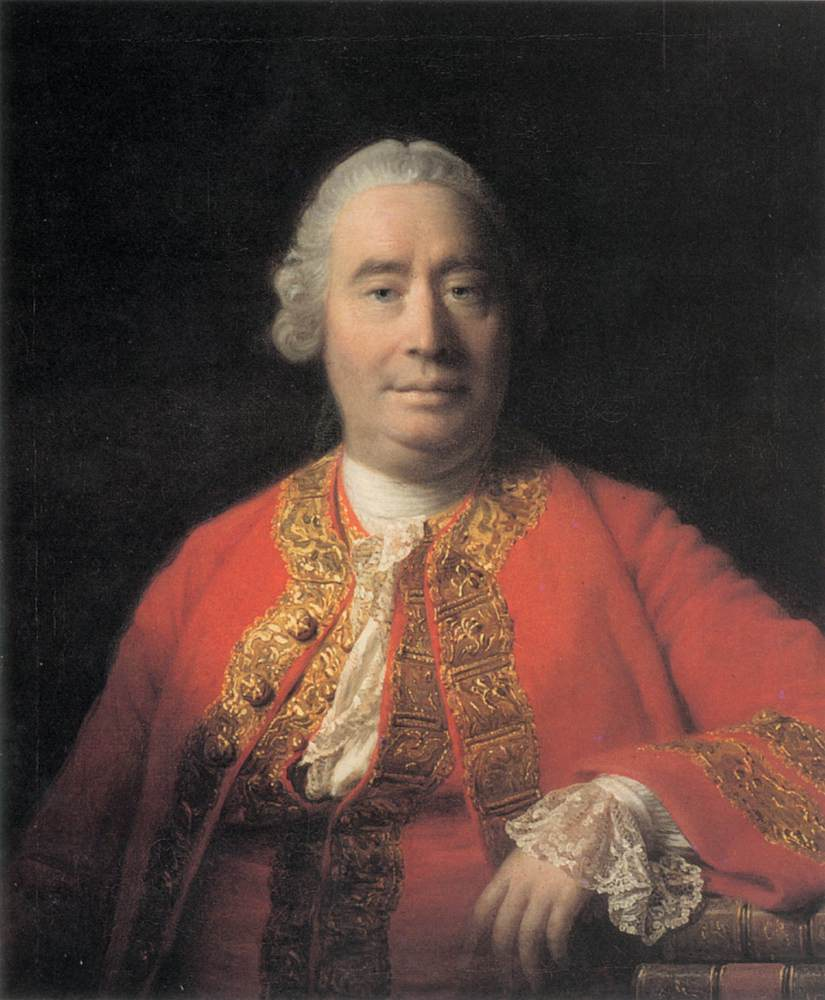
\includegraphics[height=4cm]{../../graphics/hume.jpg}
            \end{column}
            \begin{column}{7cm}
                \begin{itemize}
                    \item<1-> Natural virtues are implanted instincts involving natural dispositions to perform certain actions in certain circumstances
                    \item<2-> Every performance of the relevant action in the relevant circumstance produces some good
                    \item<3-> Artificial Virtues are not implanted instincts; they involve dispositions to behave in accordance with human convention
                    \item<4-> Not every observance of these conventions produce some good
                \end{itemize}
            \end{column}
        \end{columns}
}

% section natural_and_artificial_virtues (end)

\section{Next Time}\label{sec:next_time} % (fold)



% section next_time (end)
\end{document}
